\documentclass[a4paper,french,11pt,twoside]{VcCours}

\newcommand{\dt}{\text{d}t}
\newcommand{\dx}{\text{d}x}

\begin{document}
\Titre{PSI}{Promotion 2021--2022}{Informatique}{Devoir non surveillé n°1}
\begin{center}
\large\bf 
Pour le vendredi 19 novembre 2021, travail par deux autorisé.
\end{center}
\separationTitre


\section*{Introduction}
Une grille de Sudoku est une grille de taille $9 \times 9$, découpée en $9$ carrés de taille $3 \times 3$. Le but est de remplir cette grille avec des chiffres de $1$ à $9$ de sorte que chaque ligne, chaque colonne et chacun des $9$ carrés de tailles $3 \times 3$, contienne une et une seule fois chaque entier de $1$ à $9$. On dit dans ce cas que la grille est complète.

\medskip
En pratique, certaines cases sont déjà remplies et on fera l'hypothèse dans ce sujet que les grilles étudiées ont une unique solution.

\medskip
On représente en python en grille de Sudoku par une liste de listes de taille $9$, représentant les lignes de la grille. Les cases non remplies sont associées au chiffre $0$. Voici un exemple :

\begin{center}
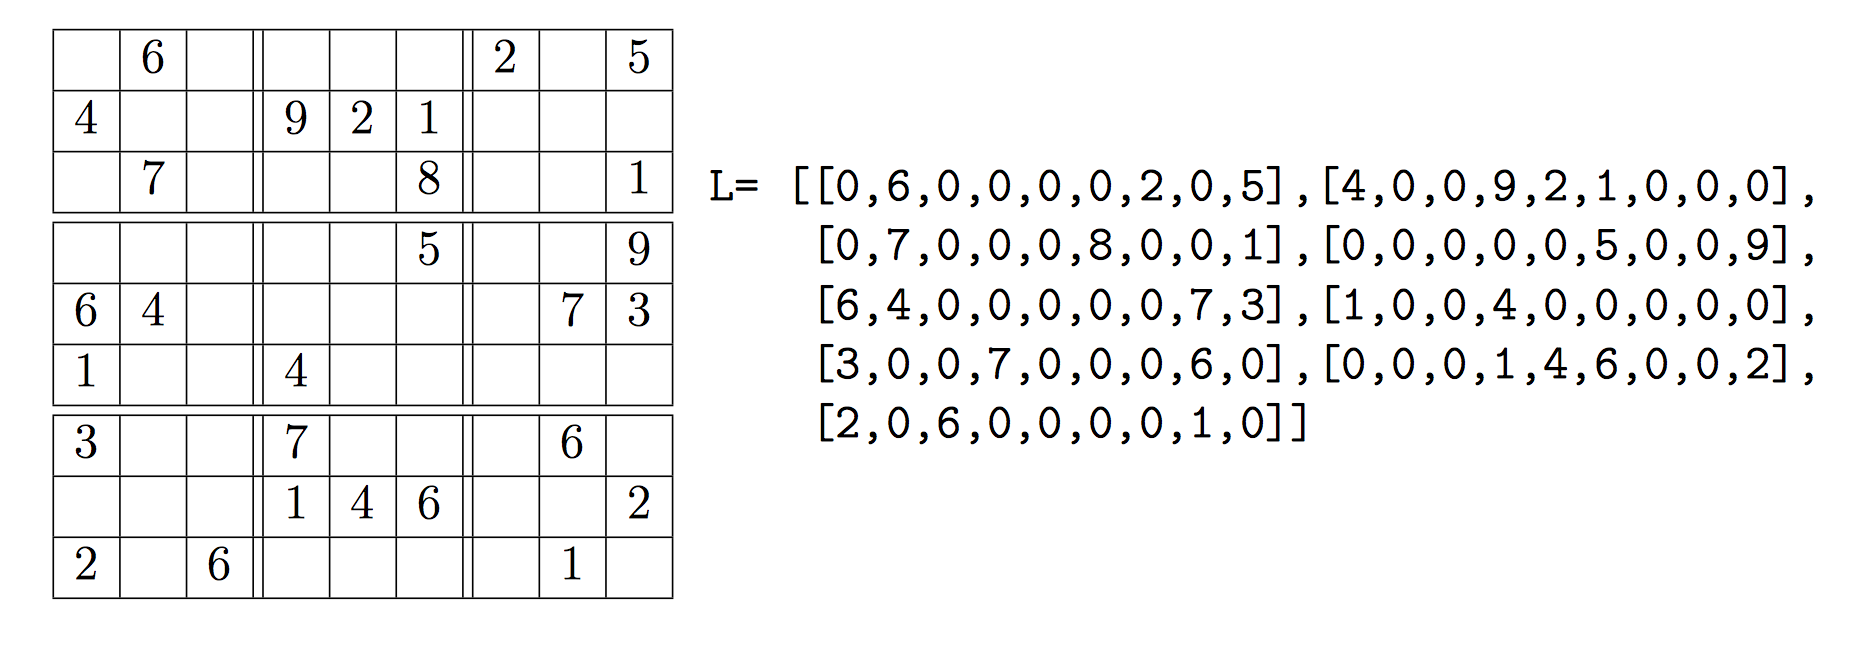
\includegraphics[scale=0.5]{Sud1}
\end{center}


Les 9 carrés de taille $3 \times 3$ sont numérotés de $0$ à $8$ du haut à gauche jusqu'à en bas à droite. Ainsi, sur la grille de l'exemple précédent, le carré $0$, en haut à gauche, contient les chiffres $6$, $4$, $7$. Le carré $1$, en haut au milieu, contient les chiffres $9$, $2$, $1$ et $8$. Le carré $8$, en bas à droite, contient les chiffres $6$, $2$ et $1$.
\begin{enumerate}
\item Comment accéder, pour $i \in \iii{0}{8}$, à la $i$-ième ligne d'une grille L?
\item Comment accéder, pour $(i,j) \in \iii{0}{8}^2$, au numéro de la case $(i,j)$ d'une grille L?
\end{enumerate}

\bigskip

\begin{center}
 \subsection*{Partie 1 : quelques fonctions utiles}
\end{center}

\medskip

\begin{enumerate}
\setcounter{enumi}{2}
\item Montrer que si une grille de Sudoku est complète alors pour chacune des lignes, chacune des colonnes et chacun des carrés de tailles $3 \times 3$, la somme des chiffres fait $45$. La réciproque est-elle vraie ?
\item Écrire une fonction {\tt ligne\_complete(L,i)} qui prend une grille de Sudoku L et entier $i$ compris entre $0$ et $8$, renvoyant {\tt True} si la ligne $i$ du Sudoku L vérifie les conditions de remplissage d'un Sudoku, et {\tt False} sinon.

\medskip

On définit de même (on ne demande pas de les écrire) les fonctions {\tt colonne\_complete(L,i)} pour la colonne $i$ et {\tt carre\_complet(L,i)} pour le carré $i$.
\item Écrire une fonction {\tt complet(L)} qui prend une liste Sudoku L comme argument, et qui renvoie {\tt True} si la grille est complète et {\tt False} sinon.
\item Compléter la fonction suivante {\tt ligne(L,i)}, qui renvoie la liste des nombres compris entre $1$ et $9$ qui apparaissent sur la ligne d'indice $i$.
\end{enumerate}

\begin{center}
\begin{minipage}{0.7\textwidth}
		
\begin{lstlisting}
def ligne(L,i):
    chiffre =[]
    for j in ...:
        if (....):
            chiffre.append(L[i][j])
    return chiffre
\end{lstlisting}

\end{minipage}
\end{center}

\medskip

Ainsi, avec la grille donnée dans l'énoncé, on doit obtenir :

\begin{center}
\begin{minipage}{0.7\textwidth}
		
\begin{lstlisting}
>>> ligne(L,0)
[6,2,5]
\end{lstlisting}

\end{minipage}
\end{center}

\medskip

On définit alors, de la même manière, la fonction {\tt colonne(L,j)} qui renvoie la liste des nombres compris entre $1$ et $9$ qui apparaissent dans la colonne $j$ (on ne demande pas d'écrire son code).


\begin{enumerate}
\setcounter{enumi}{6}
\item On se donne une case $(i,j)$ avec $(i,j) \in \iii{0}{8}^2$. Montrer que la case en haut à gauche du carré $3 \times 3$ auquel appartient la case $(i,j)$ a pour coordonnées :
$$  \left( 3 \times \left\lfloor \dfrac{i}{3} \right\rfloor , 3 \times \left\lfloor \dfrac{j}{3} \right\rfloor \right)$$
où $\lfloor x \rfloor$ désigne la partie entière d'un réel $x$.
\item Compléter alors la fonction {\tt carre(L,i,j)}, qui renvoie la liste des nombres compris entre $1$ et $9$ qui apparaissent dans le carré $3 \times 3$ auquel appartient la case $(i,j)$.
%cSpell:ignore icoin jcoin
\begin{Python}
def carre(L,i,j):
    icoin =
    jcoin =
    chiffre=[]
    for i in range(....):
        for j in range(....):
            if(....):
                chiffre.append(L[i][j]) 
    return chiffre
\end{Python}
\end{enumerate}

Ainsi, avec la grille donnée dans l'énoncé, on doit obtenir :
\begin{Python*}
>>> carre(L,4,6)
[9,7,3]
>>> carre(L,4,5)
[5,4]
\end{Python*}

\begin{enumerate}\setcounter{enumi}{8}
\item Déduire des questions précédentes, une fonction {\tt conflit(L,i,j)} renvoyant la liste des chiffres que l'on ne peut pas écrire en case $(i,j)$ sans contredire les règles du jeu. La liste renvoyée peut très bien contenir des redondances. 
\item Compléter enfin la fonction {\tt chiffres\_ok(L,i,j)} qui renvoie la liste des chiffres que l'on peut écrire en case $(i,j)$.
\begin{Python}
def chiffres_ok(L,i,j):
    ok=[]
    conflits=conflit(L,i,j)
    for k in ....:
        if ....:
            ok.append(k)
    return ok
\end{Python}
\end{enumerate}
Par exemple, avec la grille initiale :
\begin{Python*}
>>> chiffres_ok(L,4,2):
[2,5,8,9]
\end{Python*}
On pourra, dans la suite, utiliser les fonctions annexes définies précédemment.


\subsection*{Partie 2 : un algorithme naïf}
L'idée est de commencer par compléter les cases n'ayant qu'une seule possibilité. Nous prendrons dans la suite la grille suivante : 

\begin{center}
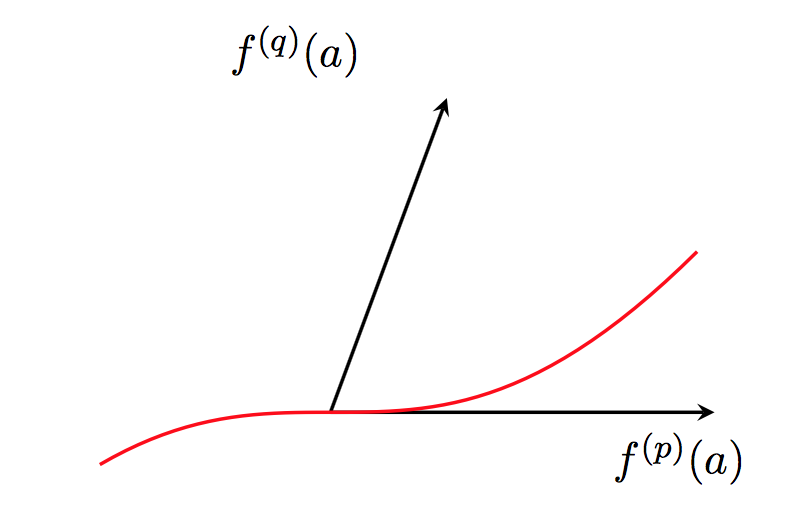
\includegraphics[scale=0.45]{im2}
\end{center}

\begin{enumerate}\setcounter{enumi}{10}
\item A partir des fonctions annexes, écrire une fonction {\tt np\_possible(L,i,j)} renvoyant le nombre de chiffres possibles à la case $(i,j)$.
\item On souhaite disposer de la fonction {\tt un\_tour(L)} qui parcourt l'ensemble des cases de la grille de Sudoku, qui complète les cases dans le cas où il n'y a qu'un chiffre possible, et renvoie {\tt True} s'il y a eu un changement, et {\tt False} sinon. La liste L est alors modifiée. Par exemple, en partant de la grille $M$ :
\begin{Python*}
>>> un_tour(M)
True
>>>M
[[2, 0, 0, 0, 9, 0, 3, 0, 0], [0, 1, 9, 0, 8, 0, 5, 7, 4],
[0, 0, 8, 4, 0, 0, 6, 2, 9], [5, 9, 0, 6, 2, 1, 4, 8, 7],
[0, 2, 7, 0, 3, 8, 1, 6, 5], [0, 6, 1, 5, 7, 4, 2, 9, 3],
[0, 8, 5, 0, 0, 9, 7, 3, 0], [9, 3, 6, 0, 5, 0, 8, 4, 2],
[0, 0, 2, 0, 6, 0, 9, 5, 1]]
\end{Python*}
On propose la fonction suivante :
\begin{Python}
def un_tour(L):
    changement=False
    for i in range(1,9):
        for j in range(1,9):
            if (L[i][j] = 0):
                if (nb_possible(L,i,j) = 1):
                    L[i][j] = chiffres_ok(L,i,j)[1]
    return changement
\end{Python}
Recopier ce code en corrigeant les erreurs.
\item Écrire une fonction {\tt complete(L)} qui exécute la fonction {\tt un\_tour(L)} tant qu'elle modifie la liste, et renvoie {\tt True} si la grille est complétée, et {\tt False} sinon.
\end{enumerate}

%cSpell:ignore backtracking
 \subsection*{Partie 3 : la méthode du backtracking}
Pour résoudre une grille de Sudoku, on va utiliser une méthode dite \og force brute \fg,
celle du \og backtracking \fg{} qui est une façon de tester toutes les possibilités de remplissage pour trouver la bonne.

\medskip

Ce n'est évidemment pas la plus rapide. Des méthodes plus proches de celles réalisées par un humain en train de résoudre la grille existent. Elles sont plus rapides, mais plus difficiles à coder.

\subsubsection*{Principe du Backtracking}
\begin{itemize}
    \item On détermine d'abord la liste des cases vides.
    \item On commence par la première case (vide) de la liste.
    \item On la rempli avec $1$ :
    \begin{itemize}
        \item Si la valeur respecte les règles, alors on passe à la case suivante.
        \item Sinon on essaie le chiffre suivant (ce qui revient à ajouter $1$ à la case)
    \end{itemize}
    \item Si aucune valeur (de $1$ à $9$) ne convient, on revient à la case (vide) 
    précédente et on essaie sur cette case le chiffre suivant.
\end{itemize}
En bref, la méthode consiste donc à essayer de remplir la grille, 
et à chaque fois que ça coince, on revient d'une case en arrière 
et on essaie le chiffre suivant. Jusqu'à ce qu'on trouve

%cSpell:ignore Lvide
\begin{enumerate}\setcounter{enumi}{13}
\item Écrire une fonction {\tt liste\_zero(L)} retournant la liste des coefficients $(i,j)$ (considérés comme des listes) de la grille {\tt L} tels que {\tt L[i,j]=0}. 
\item Écrire une fonction {\tt remplir(L,Lvide,k)} respectant les instructions suivantes :
\begin{itemize}
\item {\tt L} est une grille de Sudoku.
\item {\tt Lvide} est la liste des coefficients $(i,j)$ (considérés comme des listes) de la grille {\tt L} tels que {\tt L[i,j]=0}.
\item {\tt k} un indice compris entre $0$ et {\tt len(Lvide)-1}.
\item Cette fonction incrémente de $1$ la valeur de {\tt L[i,j]}, où $(i,j)$ est le coefficient stocké en $k$-ième position dans {\tt Lvide}, jusqu'à obtenir un chiffre qui ne contredit pas les règles du jeu (on utilisera la fonction {\tt chiffres\_ok}).
\item  Cette fonction renvoie le chiffre obtenu ou le nombre 10 si aucun chiffre ne fonctionne.
\end{itemize}
\item %cSpell:ignore resolution
Écrire alors une fonction {\tt resolution(L)} renvoyant la grille après résolution (on suppose que la grille admet une solution donc la méthode fonctionne nécessairement). On testera ce programme avec la grille suivante et on précisera  la solution.
\begin{Python*}
>>>L=[[0, 1, 3, 0, 0, 9, 0, 0, 5],
      [6, 0, 0, 0, 4, 0, 0, 0, 9],
      [4, 0, 5, 3, 0, 7, 6, 1, 2],
      [5, 0, 0, 0, 1, 3, 0, 9, 0], 
      [0, 2, 1, 7, 0, 4, 5, 8, 0], 
      [0, 4, 0, 8, 2, 0, 0, 0, 3], 
      [2, 3, 9, 0, 0, 6, 4, 0, 8], 
      [1, 0, 0, 0, 5, 0, 3, 0, 7],
      [8, 0, 0, 4, 0, 2, 0, 0, 0]]
\end{Python*}
\end{enumerate}

\end{document}